\newpage
\section{Part D}
\label{sec:sec_d}
Next, an 80:20 split was applied to the dataset and binary classifier was trained with two hidden layers of 16 and 4 neurons each. The model can be defined by the following code. 

\LST{part\_d1}

The model was trained for 50 epochs using the Adam optimize, BCELoss, and a learning rate of 0.001. Figure~\ref{fig:loss} shows the loss curve.

\begin{figure}[htpb]
	\centering
	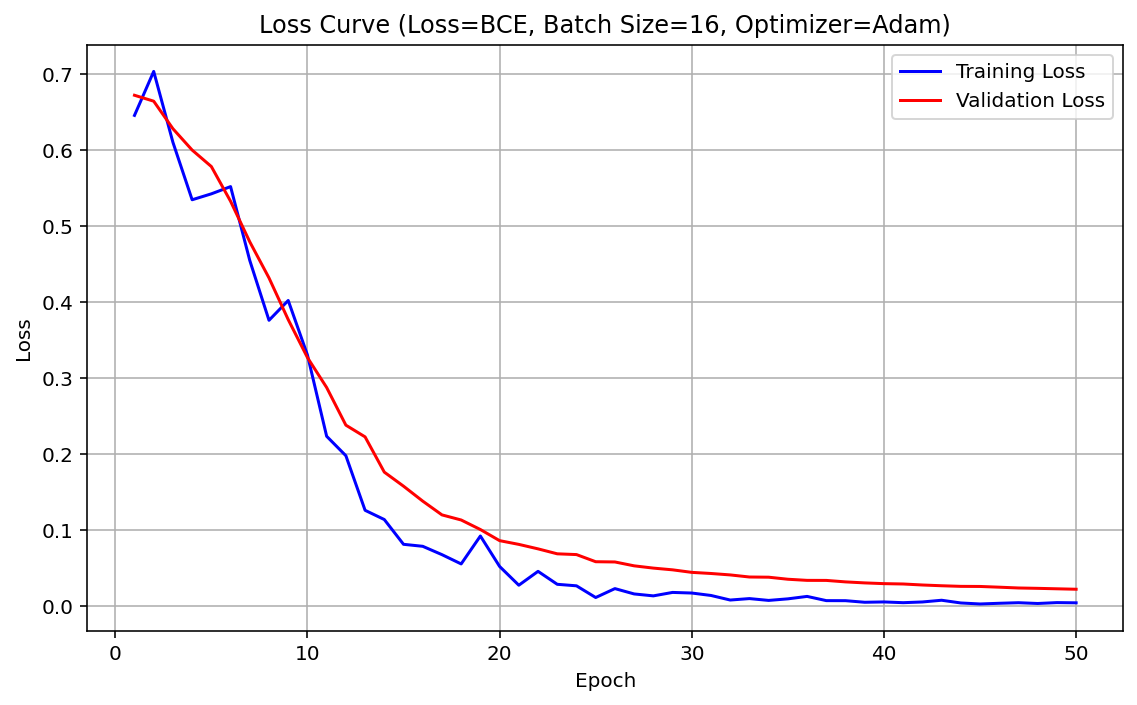
\includegraphics[width=\columnwidth]{figures/loss.png}
	\caption{Loss Curve with (\textbf{Adam}, \textbf{BCE})}
	\label{fig:loss}
\end{figure}

The for this dataset the ROC curve (Figure~\ref{fig:roc}) was found to be ideal and the TPR, FPR was computed to be $1.0$ and $0.0$ respectively for a threshold value of 0.5. The results of apply the final model to the validation set can be found in Figure~\ref{fig:val} where the title of each subplot is the model's output. 

\begin{figure}[htpb]
	\centering
	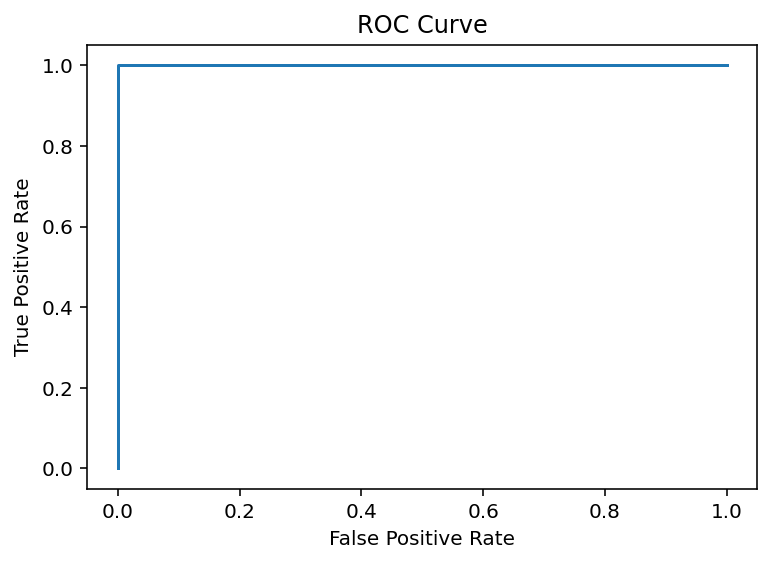
\includegraphics[width=\columnwidth]{figures/holdout.png}
	\caption{ROC Curve}
	\label{fig:roc}
\end{figure}

\begin{figure}[htpb]
	\centering
	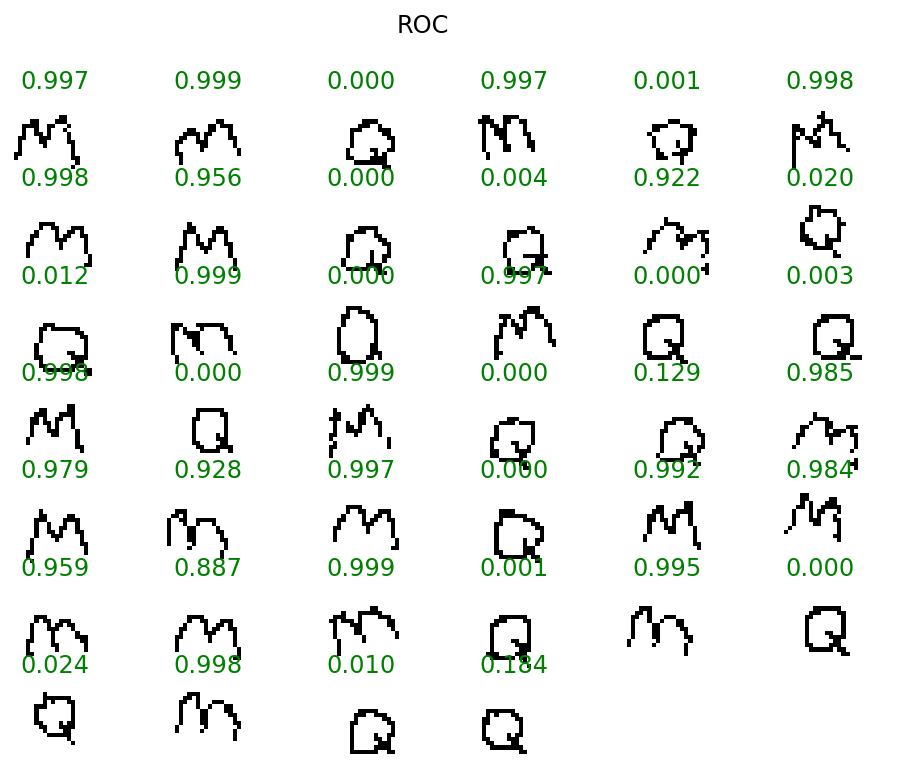
\includegraphics[width=\columnwidth]{figures/validation_results.png}
	\caption{Validation Dataset Results}
	\label{fig:val}
\end{figure}


Given that the experiment resulted perfect validation results I tested on an additional dataset to verify if it was actually learning correctly. I generated a new dataset of 5 Q's and 5 M's, these are not augmented versions of the original 20 like the training set was, they are truly unique. I applied the learned model to these and got the results shown in Figure~\ref{fig:holdout}. It can be seen that with a threshold of 0.5 the model correctly classifies all 10 new images, with reasonably high confidence values. 
\\
\begin{figure}[htpb]
	\centering
	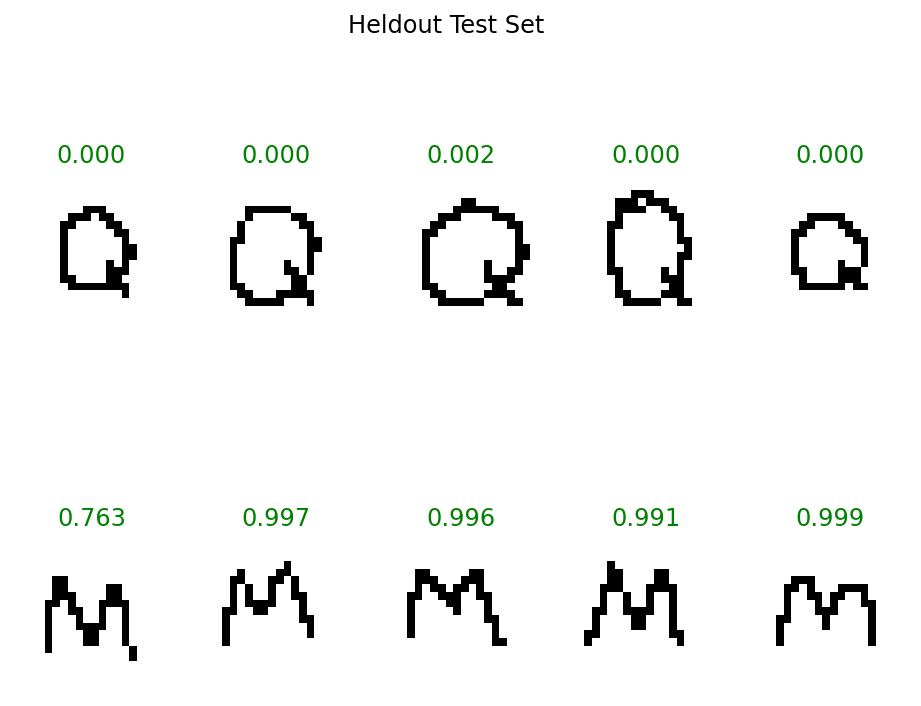
\includegraphics[width=\columnwidth]{figures/holdout_results.png}
	\caption{Holdout Dataset Results}
	\label{fig:holdout}
\end{figure}



